\documentclass[10pt]{beamer}

\usepackage[utf8]{inputenc}
\usepackage{tcolorbox}
\usepackage{tikz}
\usepackage{tikz-3dplot}
\usetikzlibrary{intersections,calc}
\usepackage{amsmath}
\usepackage{graphicx}
\usepackage{cases}
\def \heart {\textcolor{blue}{$\heartsuit$} }
\def \C {$\mathcal{C}$}
\def \orthog {\underline{\perp}}
\def\arcos{\operatorname{arcos}}

\tcbset{%
	basic/.style={colframe=black,
		      colback=white,
		      top= 0mm,
		      bottom = 2mm,
		      boxsep=0mm
		      }
}
\tikzset{
    invisible/.style={opacity=0},
    visible on/.style={alt={#1{}{invisible}}},
    alt/.code args={<#1>#2#3}{%
      \alt<#1>{\pgfkeysalso{#2}}{\pgfkeysalso{#3}} % \pgfkeysalso doesn't change the path
    },
  }

    
\begin{document}  
    \beamertemplatenavigationsymbolsempty
    \setlength{\abovedisplayskip}{0pt}
    \setlength{\belowdisplayskip}{0pt}
    \frame{
	  
	  \frametitle{Q5 Juillet 2011.}
	  %\renewcommand{\theenumi}{\alph{enumi})}
	  On considère une pyramide droite à base carrée $SABCD$ (en d’autres
	  termes, la base $ABCD$ de cette pyramide est un carré, et le pied $H$
	  de la hauteur issue de $S$ est le centre de ce carré). Cette pyramide est
	  telle que $|AB| = |SH|$.
	  Cette pyramide est également inscrite dans une sphère (c’est-à-dire que
	  les points $A, B, C, D$ et $S$ sont situés à la surface de cette sphère).
	  Si $V$ et $V'$ désignent respectivement le volume de la pyramide et de la
	  sphère, calculer la valeur du rapport $\frac{V'}{V}$ et en donner une expression
	  indépendante du rayon de la sphère et du côté de la base de la pyramide.
	  \vfill
	  
	  \pause
	  % hypothèses et thèse
	  \begin{tcolorbox}[basic] 
	      \begin{columns}[t]
		 
		 \column{.5\textwidth}\centering
		      
		      \underline{Hypothèses} 
		      \begin{itemize}
		      \item $SABCD$ pyramide à base $\square$,
		      \item $[SH]$ hauteur issue de $S$.
		      \end{itemize}

		  
		  \column{.5\textwidth}\centering
		      
		      \underline{Thèse} \\
		      \smallskip
		      $\dfrac{V'}{V}$.
		
	      \end{columns}
	  \end{tcolorbox}
    }

    \frame{ 
	  % résolution ex1
	  \begin{columns}[t]
		\column{.528\textwidth}\centering 
		

			\underline{Dessin}\\
			
				  \begin{figure}[h]
				  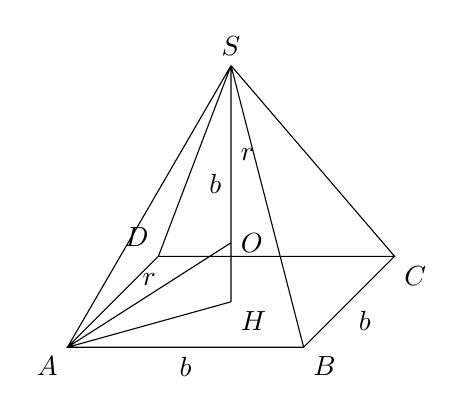
\begin{tikzpicture}[scale=0.75]
			          %projection ($(X)!(B')!(B)$)
			          %nommer chemin 'name path
			          %intersection \path [name intersections={of=d and gb,by=G}];
			          %Pyramide a base carree
			          \coordinate[label=below right:$H$](H) at (0,0,0);
			          \coordinate[label=below right:$B$](B) at (2,0,2);
			          \coordinate[label=below right:$C$](C) at (2,0,-2);
			          \coordinate[label=above left:$D$](D) at (-2,0,-2);
			          \coordinate[label=below left:$A$](A) at (-2,0,2);
			          \coordinate[label=above:$S$](S) at (0,4,0);
			          \coordinate[label=right:$O$](O) at (0,1,0);
			          \draw (A) --node[below] {$b$} (B) --node[below right] {$b$} (C) -- (D) --cycle
					(A) -- (S) (B) -- (S) (C) -- (S) (D) -- (S)
					(O) --node[above] {$r$} (A)
					(A) -- (S)
					(A) -- (H)
					(H) --node[left] {$b$} (S)
					(O) --node[right] {$r$}(S);
				  \end{tikzpicture}
				  \end{figure}
			
				  \begin{tcolorbox}[basic] 
				      
				    \smallskip
				    \underline{Hypothèses} 
				    \begin{enumerate}
				    \item $SABCD$ pyramide à base $\square$,
				    \item $[SH]$ hauteur issue de $S$.
				    \end{enumerate}
							      
				    \underline{Thèse} \\
				    \smallskip
				    $\dfrac{V'}{V}$.
				    \end{tcolorbox}
		
		
		\column{.51\textwidth}\centering
		
		\underline{Résolution}\\ \flushleft
		$O$ centre de la sphère, \\
		$r$ rayon de la sphère, \\
		$b$ longueur des côtés du carré. \\[0.05em]
		\begin{align*}
		r=&|SO|\\
		 =&|AO|=|BO|=|CO|=|DO|.
		\end{align*} \\[0.1em]
		
		\begin{enumerate}
		 \item $O \in SH$ car $SH$ est $\cap$ plans médiateurs des côtés du carré, 
		 \item $\Delta AOH$ rectangle.
		\end{enumerate}	
		$|AH|=\frac{\sqrt{2}}{2}b$,\\ \smallskip
		$|OH|=|b-r|$, \\ 
		\begin{align*}
		 |AH|^2 + |OH|^2 =& |AO|^2, \\
		 \dfrac{b^2}{2} + |b-r|^2 =& r^2,\\
		 r=& \dfrac{3l}{4}.
		\end{align*}

		
		
		
		%\centering\noindent\rule{2cm}{0.4pt}
	        %\hfill $\qed$

   
	   \end{columns}
    
    
    
    }
	
\frame{ 
	  % résolution ex1
	  \begin{columns}[t]
		\column{.528\textwidth}\centering 
		

			\underline{Dessin}\\
			
				  \begin{figure}[h]
				  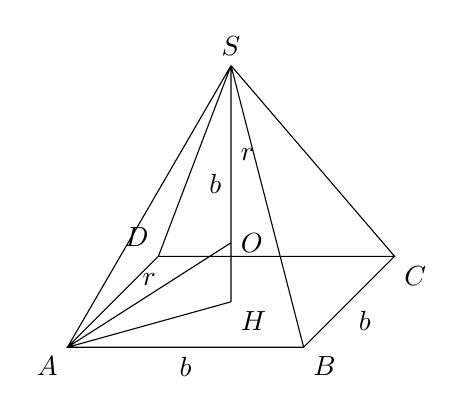
\begin{tikzpicture}[scale=0.75]
			          %projection ($(X)!(B')!(B)$)
			          %nommer chemin 'name path
			          %intersection \path [name intersections={of=d and gb,by=G}];
			          %Pyramide a base carree
			          \coordinate[label=below right:$H$](H) at (0,0,0);
			          \coordinate[label=below right:$B$](B) at (2,0,2);
			          \coordinate[label=below right:$C$](C) at (2,0,-2);
			          \coordinate[label=above left:$D$](D) at (-2,0,-2);
			          \coordinate[label=below left:$A$](A) at (-2,0,2);
			          \coordinate[label=above:$S$](S) at (0,4,0);
			          \coordinate[label=right:$O$](O) at (0,1,0);
			          \draw (A) --node[below] {$b$} (B) --node[below right] {$b$} (C) -- (D) --cycle
					(A) -- (S) (B) -- (S) (C) -- (S) (D) -- (S)
					(O) --node[above] {$r$} (A)
					(A) -- (S)
					(A) -- (H)
					(H) --node[left] {$b$} (S)
					(O) --node[right] {$r$}(S);
				  \end{tikzpicture}
				  \end{figure}
			
				  \begin{tcolorbox}[basic] 
				      
				    \smallskip
				    \underline{Hypothèses} 
				    \begin{enumerate}
				    \item $SABCD$ pyramide à base $\square$,
				    \item $[SH]$ hauteur issue de $S$.
				    \end{enumerate}
							      
				    \underline{Thèse} \\
				    \smallskip
				    $\dfrac{V'}{V}$.
				    \end{tcolorbox}
		
		
		\column{.51\textwidth} \flushleft
		\heart Volume sphère = $\dfrac{4\pi r^3}{3}$ \\ \medskip
		\heart Volume pyramide = $\dfrac{base.hauteur}{3}$ \\ \bigskip
		
		
		$$\dfrac{V'}{V} = \dfrac{27\pi}{16}$$ \hfill $\qed$
		
		

		
		
		
		%\centering\noindent\rule{2cm}{0.4pt}
	        %\hfill $\qed$

   
	   \end{columns}
    
    
    
    }
  
\end{document}
